\section{Programmtests}
\FloatBarrier

\paragraph{Erkl"arung des Toolkits}
Um effektiv Tests zum Einlesen sowie Ausgeben von Spielst"anden aus einer .txt Datei gestalten zu k"onnen, wurde eine Klasse geschrieben, welche dies erleichtern soll. Sie nennt sich \emph{TestToolkit}. Bei der Erstellung habe ich mich stark an dem Toolkit aus der "Ubung \emph{Algorithmen und Datenstrukturen} orientiert. Das gegebene Toolkit ist allerdings nur in der Lage unter einer Unix-Umgebung Dateivergleiche durchzuf"uhren, da das Programm allerdings unter Windows entwickelt wurde, mussten viele Methoden ausgetauscht werden. Die Datei aus Algorithmen und Datenstrukturen befindet sich ebenfalls im Verzeichnis des Anhangs, kann aber auch wieder alternativ "uber die Lesezeichen- bzw. die Anlage"ubersicht betrachtet werden. 

\embedfilesetup{mimetype=text/x-java-source,java}
\embedfile{programmierhandbuch/programmtests/TestToolkit.java}

Neben einer Festlegung welcher Dateityp bearbeitet werden kann, liefert diese Klasse vor allem einen Pfad an dem s"amtliche Testdateien zu finden sind. Dies geschieht ("ahnlich wie beim Logger) mit einem Formatstring. Um Testdateien zuallererst in Form eines Strings zu lesen wird die Methode \emph{readAsString} verwendet \lstref{lst:testToolkit_readAsString}. Diese verwendet allerdings nur die bereits implementierte Methode der Loader-Klasse. Es war mir trotzdem wichtig sie hier mit aufzunehmen, um eine gemeinsame Schnittstelle f"ur alle Tests der Dateiverarbeitung zu schaffen. In der Methode \emph{read} wird diese Methode aufgerufen um einen Game Konstruktor zu f"ullen und ein vollwertiges Spiel zur"uckzugeben. 

Eine weitere Funktionalit"at des Toolkits besteht darin zwei gegebene Dateien mit dem selben Namen auf ihre Gleichheit zu pr"ufen \lstref{lst:testToolkit_assertFilesEqual}. Dies geschieht, indem beide Dateien aus den gegebenen Verzeichnissen (\emph{results} sowie \emph{expected\_results}) als Strings ausgelesen und anschlie"send per assertEquals verglichen werden. Die Methode \emph{writeAndAssert} verh"alt sich hier sehr "ahnlich, hierbei wird nur erst das gegebene Spiel in eine Datei geschrieben bevor die assertFilesEqual der Klasse aufgerufen wird. 
\begin{lstlisting}[float,style=CodeHighlighting,caption=TestToolkit - readAsString,label=lst:testToolkit_readAsString]
public static String readAsString(String filename) {
    try {
        File file = new File(String.format(PATH_FORMAT, filename));
        return Loader.getInstance().openGivenFile(file.getPath());
    } catch (FileNotFoundException e) {
        return e.getMessage();
    }
}
\end{lstlisting}
\begin{lstlisting}[float,style=CodeHighlighting,caption=TestToolkit - assertFilesEqual,label=lst:testToolkit_assertFilesEqual]
public static void assertFilesEqual(String filename) {
    try {
        File fileResult = new File("test" + File.separator + "fileTests" + File.separator
                + "results" + File.separator + filename + ".txt");
        File fileExpectedResult = new File("test" + File.separator + "fileTests" 
        		+ File.separator + "expected_results" + File.separator + filename 
        		+ ".txt");
        Assert.assertEquals(Loader.openGivenFile(fileExpectedResult), 
        		Loader.openGivenFile(fileResult));
    } catch (FileNotFoundException e) {
        assertTrue(false);
    }
}
\end{lstlisting}

\subparagraph{Beschreibung der Testf"alle}
Im Ordner namens \glqq test\grqq befindet sich ein Unterordner namens \glqq fileTests\grqq {}. Dies ist der Oberordner, in welchem sich alle Testdateien zum Dateieinlesen sowie ausgeben befinden. Die Dateien mit dem Pr"afix \glqq inv\_\grqq {} spiegeln invalide, w"ahrend die mit dem Pr"afix \glqq val\_\grqq {} valide Dateien wiederspiegeln. Da im Converter drei unterschiedliche Komponenten generiert werden, wurden die Testf"alle hieran angelehnt. Es gibt also jeweils Testf"alle f"ur Fehler im Spielbrett, den B"anken und dem Stapel. Zu validen Spielsituationen gibt es deutlich weniger Tests, da viele der Situationen in den Unittests zu den einzelnen Datenstrukturen bereits behandelt wurden. Invalide Dateitests laufen immer nach dem selben Schema ab \lstref{lst:test_noTagOpenerAtBeginningOfDoc}. Es wird die erwartete Fehlermeldung in eine Variable gespeichert. Anschlie"send wird der String aus der Datei mittels \emph{readAsString} aus der Toolkit-Klasse gelesen und dem Converter "ubergeben um dieselbe Situation zu erzeugen wie es beim Einlesen im normalen Spielverlauf der Fall ist. Im letzten Schritt werden String-Ausagbe mit der Fehlermeldung vom Anfang verglichen. 

Etwas komplexer gestalten sich die Tests bez"uglich der validen Spielsituationen. Hierbei wird ein Spiel mit den erwarteten Daten erzeugt. Danach wird die Methode \emph{read} der TestToolkit-Klasse verwendet um ein Spiel zu erzeugen. Diese wurde bereits im vorherigen Absatz erw"ahnt, denn sie ruft lediglich die readAsString-Methode auf, um den generierten String dem Game-Konstruktor zu "ubergeben. Wie der Einleseprozess im Detail funktioniert wird in der Erkl"arung der Converter-Klasse beschrieben (siehe Abschnitt \ref{spar:converter_ablauf}, S. \pageref{spar:converter_ablauf}). Das so generierte Spiel wird mit einem Spiel verglichen, welches vorher \glqq per Hand\grqq {} erzeugt wurde. Hierzu wird die \emph{equals}-Methode der \emph{Game}-Klasse verwendet, welche "uber assertEquals angesteuert wird. Im Anschluss wird das gelesene Spiel einmal abgespeichert und per \emph{writeAndAssert} von der TestToolkit-Klasse "uberpr"uft ob die Datei den selben Spielstand enth"alt. In der \emph{writeAndAssert}-Methode wird zuerst eine neue Datei mit dem gegebenen Namen in dem Unterordner \glqq results\grqq  erstellt. Anschlie"send ist der Loader zum Abspeichern zust"andig. Wie der Loader vorgeht um eine Datei abzurufen wird im Abschnitt \ref{par:loader}, S. \pageref{par:loader} n"aher erl"autert. 

\subparagraph{Auflistung wichtiger Testf"alle}

\begin{tabular}{lll}
\toprule
Testf"alle\\
\midrule
Testfall & erwartetes Ergebnis & erzieltes Ergebnis\\
\midrule
test & asdf & abc\\
\bottomrule
\end{tabular}
\label{tab:testfaelle}

\todo{Tabelle unvollstaendig}

\begin{figure}
	\centering
	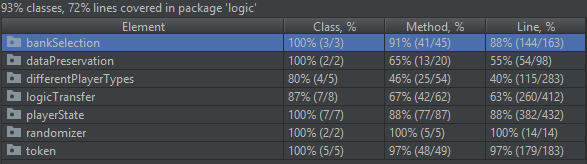
\includegraphics{pics/testCoverage}
	\caption{Testconverage}
	\label{fig:testCoverage}
\end{figure}


\begin{lstlisting}[float,style=CodeHighlighting,caption=InvalidFileReadTests - test\_noTagOpenerAtBeginningOfDoc,label=lst:test_noTagOpenerAtBeginningOfDoc]
@Test
public void noTagOpenerAtBeginningOfDoc() {
    String expOutput = WrongTagException.DEFAULT_MESSAGE;
    String fileOutput = TestToolkit.readAsString("inv_noTagOpenerAtBeginningOfDoc");
    String actOutput = new Converter().readStr(new FakeGUI(), fileOutput);
    assertEquals(expOutput, actOutput);
}
\end{lstlisting}